% !TEX root = 0_main.tex
\chapter{Evaluation}
We use a variety of benchmark functions to evaluate the performance and practicability of \sys{}.
In this section, we first describe our experimental setup (\sect{sect:exp}) and metrics for quantifying the performance of \sys{} (\sect{ssec:metrics}).
We outline the performance comparison of \sys{} (with HDL synthesizer and our custom libraries) on combinational benchmark functions with PCF \cite{kreuter2013pcf}, one of the best known earlier automated methodologies to generate circuits for garbling in \sect{ssec:customlib}.
\sys{}'s performance in generating sequential circuits for benchmark functions using a standard HDL synthesis tool is demonstrated in \sect{ssec:seqeval}.
\sect{ssec:cacheTime} shows the CPU time for various numbers of sequential cycles which demonstrates the effect of memory footprint reduction in garbling time.
\sect{ssec:HLSeval} shows a comparison between \sys{}'s performance using an HLS tool (input written in C) and using a conventional HDL synthesis tool (input given in Verilog).
Lastly, \sect{ssec:mipsres} shows the result of our garbled processor and implementation of Hamming distance as a benchmark.

We also compare the performance of the commercial logic synthesis tool with the academic, open-source tools in Appendix \ref{app:seqos}.
We show that in most cases, the performance of the open-source tool is comparable to the commercial tool.

\section{Experimental Setup}
The circuit generations are all done on a system with Linux RedHat Server 5.6, 8~GB of memory, and Intel Xeon X5450 CPU @ 3~GHz.
We use another system with Ubuntu 14.10 Desktop, 12.0~GB of memory, and Intel Core i7-2600 CPU @ 3.4GHz to assess the timing performance of the sequential garbling scheme in \sect{ssec:cacheTime}.

Two sets of HDL synthesis tool chains are used in our experiments: one commercial and one open-source (Appendix \ref{app:seqos}).
Our commercial HDL level synthesis tool is Synopsis Design Compiler (DC) 2010.03-SP4 \cite{tool:DesignCompiler}.
We also use the Synopsis Library Compiler from the DC package to interpret our custom technology library.
In \sect{ssec:HLSeval}, we utilize Xilinx Vivado HLS \cite{tool:Vivado}, a commercially available HLS tool whose inputs are written in the C/C++ programming language.
We emphasize that \sys{} can operate with any commercial or open-source sequential HDL-level (or HLS) synthesizer, as long as the synthesizer is capable of performing state-of-the-art logic optimization and mapping algorithms.

\section{Performance Metrics}
We use the following metrics to measure the efficiency of \sys{} for generating garbled circuits:

\begin{itemize}
\item
	\textit{Memory Footprint Efficiency} ($\mathit{MFE}$): $$\mathit{MFE} = \dfrac{q_{0}}{q},$$ where $q_{0}$ is the total number of gates in the reference circuit and $q$ is the total number of gates in the circuit under evaluation.
	The maximum number of tokens that need to be stored at any point during garbling/evaluation as well as memory required for storing circuit description is directly proportional to the number of gates in both sequential and combinational circuits.
	Thus, the total number of gates is approximately proportional to the memory footprint.

\item
	\textit{Number of Garbled Tables} ($\mathit{\#GT}$): $$\mathit{\#GT} = \#nonXOR\times c,$$ where $\#nonXOR$ is the number of non-XOR gates in a circuit and $c$ is the number of sequential cycles that the circuit needs to be garbled/evaluated.
	In free XOR-based GC schemes, each non-XOR gate requires a garbled table to be generated by the garbler and sent to the evaluator at each sequential cycle.
	Thus, this metric is an estimate of both the computation and communication time.

\item
	\textit{Garbled Tables Difference} ($\mathit{GTD}$ (\%)): $$\mathit{GTD} = \dfrac{\mathit{\#GT} - \mathit{\#GT}_{0}}{\mathit{\#GT}_{0}} \times 100,$$ where $\mathit{\#GT}_{0}$ is the total number of garbled tables for the reference circuit and $\mathit{\#GT}$ is the total number of garbled tables for the circuit under evaluation.
	When comparing a sequential with a combination circuit, positive $\mathit{GTD}$ shows an \emph{overhead} (caused by folding a circuit with an asymmetric loop, see \sect{sec:sequen}) in total computation and communication time resulting from an excessive number of garbled tables generated in the sequential circuits.
	However, in general, negative $\mathit{GTD}$ shows improvement in the number of non-XOR gates and generated garbled tables that results from logic synthesis optimization.
\end{itemize}

\section{Benchmark functions}
We evaluate \sys{}'s circuit generation method on various benchmark functions.
Several of these functions have been used in previous works, e.g., PCF~\cite{kreuter2013pcf}.
In the following, we introduce our benchmarks and explain how we fold them into a sequential representation.

\textit{Sum.} This function receives two $N$-bit inputs and outputs an $N$-bit sum.
The sum function is implemented in $N$ steps of one bit sums by keeping the carry bit.
Thus, it can be folded up to $N$ times without any significant overhead in number of garbled tables ($\mathit{\#GT}$).

\textit{Hamming Distance.} This function receives two $N$-bit inputs and outputs the $\log_2(N)$-bit Hamming distance between them.
The Hamming distance between two numbers is the number of positions at which the corresponding bits are different.
A possible combinational implementation of the $N$-bit Hamming distance uses a binary tree of adders that sums all $1$-bit values from the bit differences to a final Hamming distance consisting of $\log_2(N)$ bits \cite{boyar2006concrete}.
This implementation cannot be folded easily.
However, we can fold this function into $N$-cycles of one XOR and one $\log_2(N)$-bit adder.
This causes an overhead compared to the combinational circuit.

\textit{Compare (Millionaires problem).} This function receives two $N$-bit unsigned input values and outputs a greater than signal consisting of one bit that indicates if the first input is greater than the second one.
The comparison function can be implemented in $N$ steps of subtraction by keeping the carry bit \cite{kolesnikov2009improved}.
Thus, it can be folded up to $N$ times without any significant overhead.

\textit{Multiplication.} This function receives two unsigned $N$-bit inputs and outputs their unsigned $N$-bit product.
The multiplication function consists of $N$ additions and shifts.
The shift operations result in an asymmetric structure in this function.
Thus, folding it up to $N$ times may increase the overhead.

\textit{Matrix Multiplication.} This function receives two $N\times N$ matrices consisting of $32$-bit unsigned numbers and outputs an $N\times N$ matrix equal to the product of the input matrices.
The $N\times N$ matrix multiplication function consists of three $N$-cycle nested loops with a symmetric structures.
It can be folded up to $N^3$ times without any significant overhead.

\textit{AES-128.} This function receives a 128-bit plaintext and 128-bit round keys and outputs a 128-bit ciphertext based on the Rijndael algorithm.
The AES-128 function consists of 10 rounds with almost symmetric structure.
Ideally, it can be folded up to $10$ times without any significant overhead.

\textit{SHA3.} This function receives $576$-bit inputs and outputs a $1600$-bit number equal to the SHA3 hash of the input.
We implement the Keccak-f permutations[$1600$] procedure for realizing this function.
The SHA3 function consists of 24 steps, each with a symmetric structure.
It can be folded 24 times without any significant overhead.

\section{Combinational Garbled Circuit}
To show the performance gain of using our custom libraries, we compare \sys{} combinational circuits with circuits reported in PCF \cite{kreuter2013pcf}.
We choose PCF because among the \emph{automated} GC tools available at the time of writing, it shows better results for most of the benchmarks.
In some other work like FastGC \cite{huang2011faster}, a number of benchmark circuits have been more aggressively improved (compared to PCF) using ad-hoc and mostly manual optimizations, but without a generalizable methodology.

The comparison is shown in \tab{table:result-comb}.
We compute the garbled tables difference $\mathit{GTD}$ (see \sect{ssec:metrics}) of various benchmarks by using circuits reported in PCF as reference ($\mathit{GTD}$\textsuperscript{PCF}).
It can be seen that the combinational circuits generated by \sys{} have non-positive $\mathit{GTD}$\textsuperscript{PCF} which means that the number of garbled tables are less than or equal to that of PCF circuits.
We also compare the memory footprint by computing the memory footprint efficiency $\mathit{MFE}$ with PCF as reference ($\mathit{MFE}$\textsuperscript{PCF}).
We observe that $\mathit{MFE}$\textsuperscript{PCF} is larger than 1 (up to 9.3).
This means that even without using sequential circuits, the memory footprint can be reduced by almost an order of magnitude by using \sys{} custom libraries and standard HDL synthesis.

In case of Hamming distance, \sys{} shows, on average, $80\%$ improvement in number of garbled tables.
Another automated tool CBMC-GC \cite{franz2014cbmc} reports better result compared to PCF for Hamming 160 (non-XOR $\numprint{4738}$, total gates $\numprint{20356}$).
However, \sys{} shows $66\%$ improvement in number of garbled tables compared to CBMC-GC.
In case of 256-bit and 1024-bit Multiplication, and $8\times 8$ and $16\times 16$ Matrix Multiplication, because of the huge (impractical) sizes, Synopsis DC was unable to generate the entire combinational circuit.
This is because Synopsis DC is a tool developed for commercial applications.
The real-life applications are almost always written sequentially, otherwise the design would not be scalable or even amenable to offline compilation onto a hardware circuit.
We emphasize that our sequential circuit ($c>1$) provides the exact same functionality while having a very small memory footprint compared with the reference circuit.

\subsection{Comparison with Hand-Optimized Circuits}
The netlists generated by the automated flow of \sys{} show similar performance as the hand-optimized netlists in many cases.
For example, \cite{kolesnikov2009improved} describe an $N$-bit sum circuit with $5N$ gates of which $N$ gates are non-XOR and an $N$-bit comparison circuit with $4N$ gates of which $N$ gates are non-XOR.
The circuits generated by \sys{} have about the same number of gates for these two functions.
Note that one can always add any hand-optimized module to the synthesis library of \sys{}.

\section{Sequential Garbled Circuit}
As described in \sect{sec:sequen}, the user has the degree of freedom to fold a combinational circuit and convert it to a sequential one to reduce the memory footprint.
$c$ denotes the number of sequential cycles required to garble/evaluate the circuit.
This value demonstrates the amount of folding that is performed before the circuit is input to the synthesizer.
The user defines the value of $c$ and writes her own input function in an HDL or a higher level language such that the function is evaluated in $c$ sequential cycles.

We use Memory Footprint Efficiency ($\mathit{MFE}$), to evaluate the reduction in memory requirement.
We use \sys{} combinational circuits ($c=1$) as reference.
The ideal $\mathit{MFE}$ for a circuit with $c$ sequential cycles is $c$.
We also compare the memory footprints of sequential circuits with combinational circuits reported in PCF ($\mathit{MFE}$\textsuperscript{PCF}).

As explained in \sect{ssec:sqcirc}, the folding process may introduce some overhead on the total number of garbled tables.
To assess this overhead, we compute the Garbled Tables Difference ($\mathit{GTD}$) of the sequential circuit using \sys{} combinational circuits as reference.
The ideal $\mathit{GTD}$ is $0\%$, which means that the total number of garbled tables should be equal to those for a functionally equivalent combinational circuit.
We also compare the number of garbled tables of sequential circuits with combinational circuits reported in PCF ($\mathit{GTD}$\textsuperscript{PCF}) to show that even with the incurred overhead, the number of garbled tables for sequential circuits is still less than that of PCF for most cases.

\begin{table*}
\centering
\caption{Comparison of \sys{} combinational circuits with PCF.
In case of AES 128, the result is compared with FastGC.}
\label{table:result-comb}
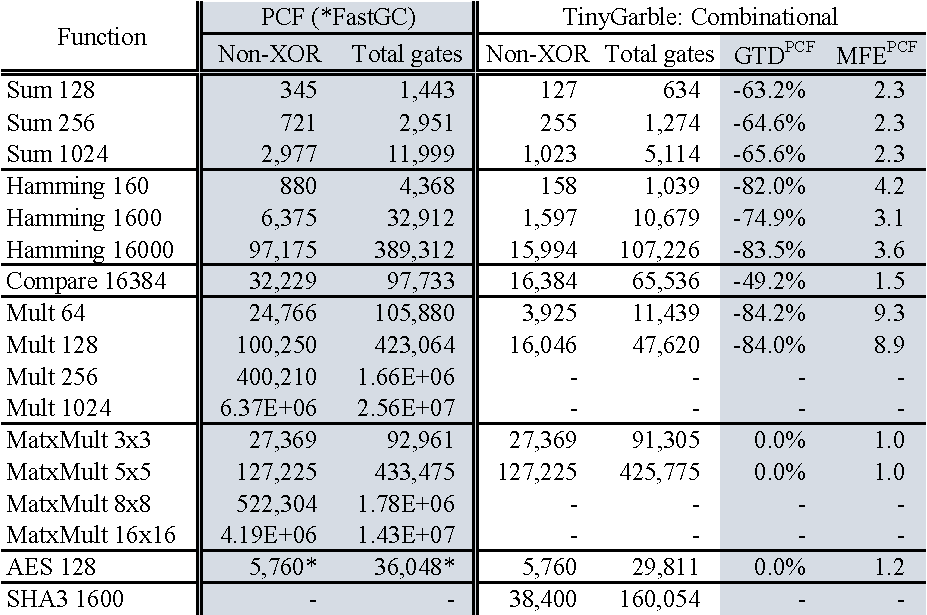
\includegraphics[scale=0.9]{results-comb-crop.pdf}
\end{table*}

\begin{table*}
\centering
\caption{Comparison of \sys{} sequential circuits with PCF and \sys{} combinational circuits.
In case of AES 128, the result is compared with FastGC.}
\label{table:result-seq}
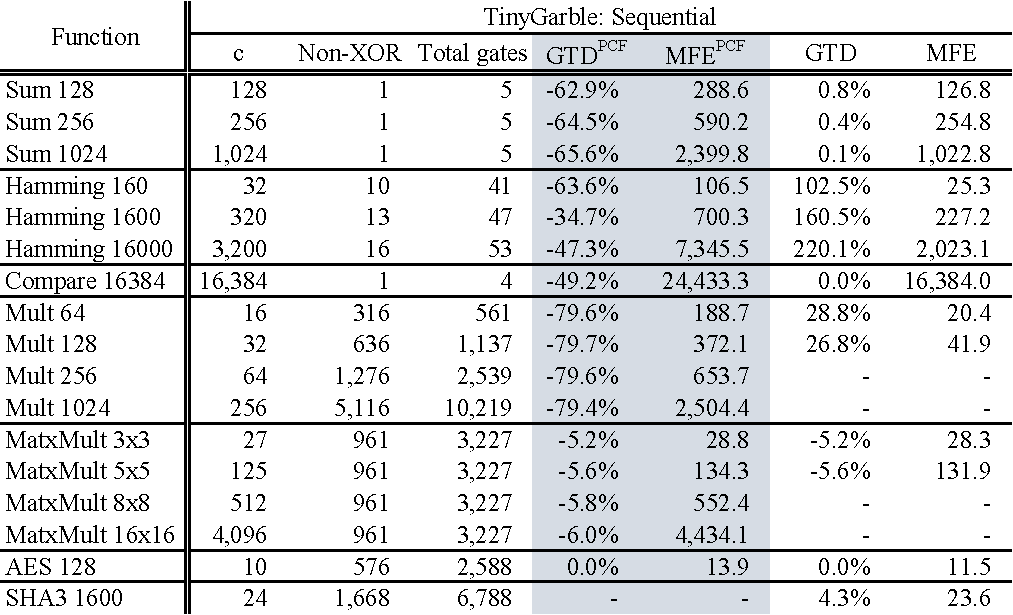
\includegraphics[scale=.9]{results-seq-crop.pdf}
\end{table*}

\tab{table:result-seq} shows the number of total gates, non-XOR gates, $\mathit{MFE}$, $\mathit{GTD}$, $\mathit{MFE}$\textsuperscript{PCF}, and $\mathit{GTD}$\textsuperscript{PCF} of the benchmark circuits for various input widths.
$\mathit{MFE}$, $\mathit{GTD}$ are computed with \sys{} combinational circuits (with $c=1$) as reference.
$\mathit{MFE}$\textsuperscript{PCF}, and $\mathit{GTD}$\textsuperscript{PCF} use the circuits reported in PCF as reference.
In the case of AES 128, we compare our implementation with the manually optimized circuit reported in FastGC \cite{huang2011faster} because PCF did not report it directly.

We provide a few highlights from \tab{table:result-seq}.
\sys{} is able to decrease the size of the sum of two $1024$-bit numbers by $\numprint{1022.8}$ times (i.e., more than three orders of magnitude) without affecting the number of garbled tables ($\mathit{GTD}$) compared with its own combinational circuit.
For Hamming 16000, \sys{} is able to decrease the memory footprint by $\numprint{7345.5}$ times (i.e., about 4 orders of magnitude) while reducing the number of garbled tables by $47.3\%$ in comparison with the circuit reported in PCF.
In case of Mult 1024, \sys{} shrinks the memory footprint by a factor of $\numprint{2504.4}$ while reducing the number of garbled tables by $79.4\%$ when compared with the result in PCF.
For a $16\times 16$ matrix multiplication, a $\numprint{4434.1}$ more compact \sys{} solution with $6\%$ less garbled tables compared with PCF is available.
By folding AES-128 10 times, the total number of gates is reduce by a factor of $13.9$ compared to the  FastGC circuit without any overhead in the number of non-XORs.
Observe that the savings are typically more for larger bit-widths while extreme foldings can introduce an increased overhead in number of garbled tables due to the resulting asymmetry.

Because of the \sys{} superior scalability, we are able to implement functions that have never been reported before, such as SHA-3, which can be represented using $\numprint{344059}$ and $\numprint{6788}$ gates respectively.

\section{Effect of Folding on Garbling Time}
So far, we have only reported the overhead in terms of garbled tables ($\mathit{GTD}$) that is a function of the number of non-XOR gates.
As explained in \cite{bellare2013efficient}, if we see garbling as a cryptographic primitive, its computation time (without considering communication) will also be interesting.
In practice, smaller circuits which can fit entirely in the processor cache result in fewer cache misses and therefore, consume less CPU cycles for garbling.
To better observe the impact of cache speed-up for the compact circuits resulting from \sys{}, \fig{fig:cpu_time} depicts the CPU Time (left y-axis) and the memory footprint of wire tokens (right y-axis) versus $c$ (x-axis) for the $\numprint{32768}$-bit Sum function.
As mentioned earlier, the memory footprint is directly proportional to the total number of gates in the sequential circuit.

This experiment is done using our sequential garbling scheme based on JustGarble \cite{bellare2013efficient} that includes using Free XOR, Row Reduction, and Fixed-key AES garbling techniques (see \sect{subsec:preli_GC}).
We use an Intel Core i7 CPU @ 3.40GHz which supports the AES-NI instruction set.
The CPU cycle is measured as the average of $10,000$ trials using RDTSC instruction.
For security parameter $k=128$ (the bit-width of wire token, see \sect{subsec:preli_GC}), we store $128$-bit per tokens.
For garbling in JustGarble, we store 2 tokens, 2 32-bit input indexes, and an 8-bit gate-type per gate.
Thus, the memory footprint is approximately $328$-bit per gate in garbling operation.
Folding the circuit by a factor of $c \in [1:\numprint{32768}]$ constantly decreases the memory footprint while the computation effort remains almost constant.
Interestingly, as can be seen from the figure, the number of CPU cycles sharply decreases by $1.6\times$ just when we fold four times ($c=4$) compared to $c=1$.
This is because for $c \geq 4$, the memory space required for garbling completely fits in the cache.
The minimum CPU cycle per gate happens at $c=\numprint{2048}$ for $3.2$~KB memory footprint.
This signifies the fact that even for large functions, we can use the sequential approach to fit the corresponding memory space requirement into the cache and avoid the penalty of cache misses, thus achieving a large reduction in garbling time.

\begin{figure}[ht]
	\centering
	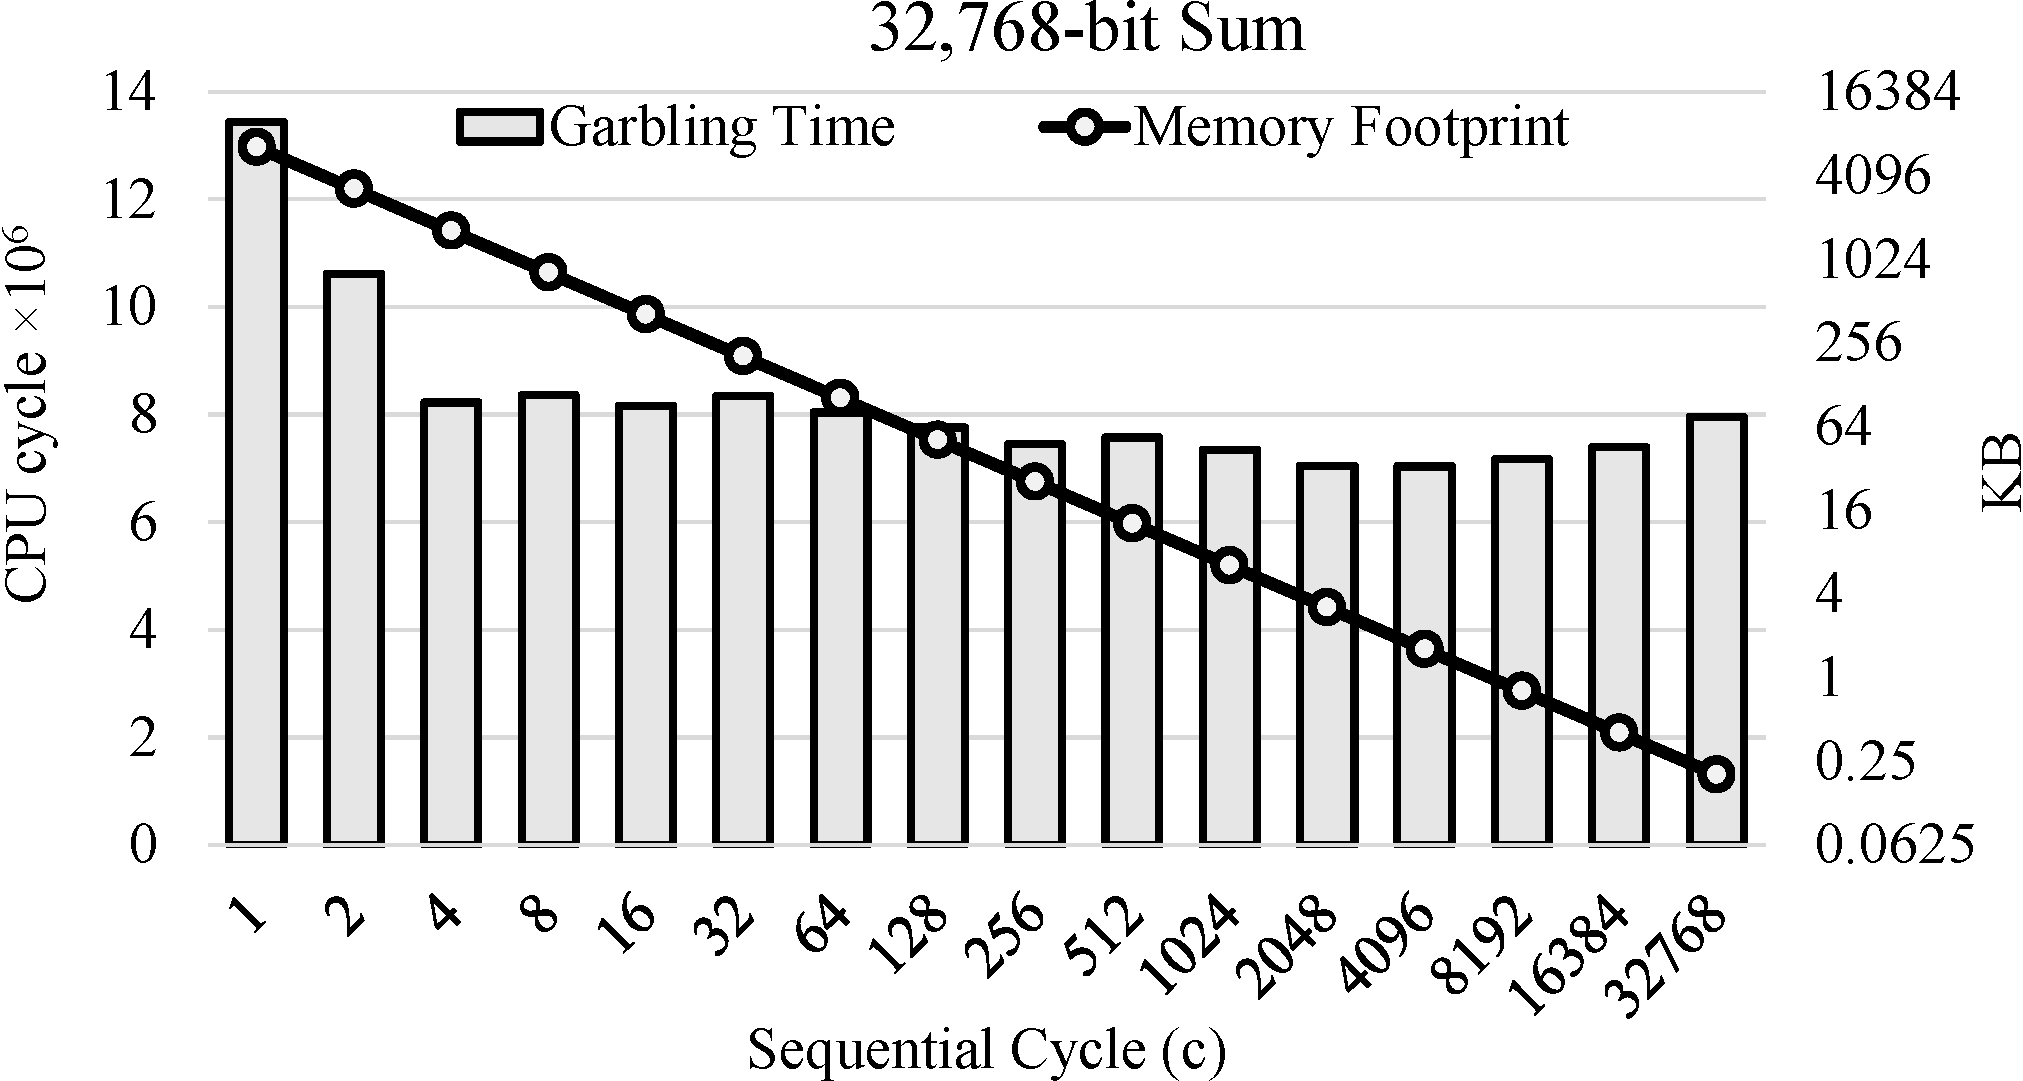
\includegraphics[width=0.7\textwidth]{CPU_Time-crop.pdf}
	\caption{Garbling $\numprint{32768}$-bit Sum function.
The CPU time in number of cycles and the approximate memory footprint in KBytes (y-axis) versus $c$ (x-axis) are shown.}
	\label{fig:cpu_time}
\end{figure}

\section{High Level Synthesis Tools}
The design automation community has been working on tools that work with higher-level languages and abstractions than HDL.
While a host of commercial and academic HLS tools are available \cite{tool:Vivado, tool:PandA, decaluwe2004myhdl, Gupta2004}, we selected the Xilinx Vivado HLS for compiling C code to HDL which can then be synthesized using a conventional HDL synthesis tool.
The HLS engine in the Vivado suite is built upon the xPilot project \cite{Chapter:Zhang2008}.

\begin{table*}[t]
\centering
\caption{Comparison of performance of the circuits generated using C input to HLS and a direct Verilog input to the HDL synthesizer.}
\label{table:hls}
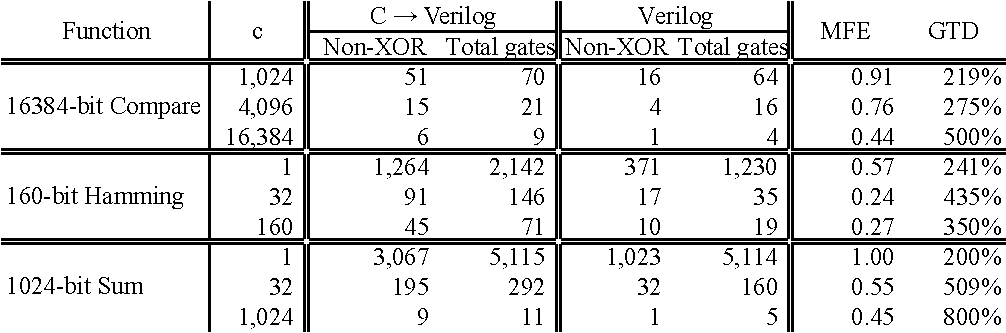
\includegraphics[scale=.9]{HLS-crop.pdf}
\end{table*}

Table \ref{table:hls} demonstrates a comparison between the performance of the circuits generated using C input to the HLS tool (C$\rightarrow$Verilog) and a direct Verilog input.
As can be seen from the table, the resulting memory footprint could increase by a factor between 1 and 4, while the number of garbled tables varies in a range of 3 to 9 times.
It is well known that writing the HDL level code which contains the time information and more detailed structural/behavioral description would yield much more efficient circuits than the code written in a higher level language.

\section{Evaluation of MIPS}
We implement general purpose processor for PF-SFE using MIPS~I where one user provide function description in assembly and the other provides the data.
Support of sequential circuits in \sys{} enables us to use the MIPS circuit description in Plasma project \cite{rhoads2006plasma} without major modifications.
In the following, we provide the result of MIPS implementation and its memory footprint and communication load.
Lastly, we present implementation of Hamming distance with variable input length as a benchmark of private function application on MIPS.

\subsection{MIPS Implementation}
We used \sys{} to generate the netlist for the MIPS sequential circuit.
\tab{table:mipsres} shows the total number of gates and non-XOR gates for each module of the MIPS processor with $64\times32$bit DM and IM.
The sum of non-XORs for each module is $\numprint{14997}$.
However, when the modules are combined together to form the entire MIPS processor, the synthesizer optimizes the circuit such that the total number of non-XORs is reduced by $14.95\%$ to $\numprint{12755}$.
The memory footprint for storing tokens during garbling MIPS is approximately the size of two tokens times the total number of gates which is $2 \times 128 \times \numprint{31719}$bit $=991$~KB for token bit-width $k=128$.
The communication load between parties for invocation of one instruction (one sequential cycle) is approximately the size of three tokens times the number of non-XOR gates which is $3\times 128 \times \numprint{12755}$bit $=598$~KB with Row Reduction optimization.

\begin{table}[h]
\centering
\caption{Number of total gates and non-XOR gates in the MIPS implementation.
The global optimization of \sys{} reduces the overall number of gates compared to that of the sum of individual modules.}\label{table:mipsres}
\resizebox{0.4\textwidth}{!}{%
\begin{tabular}{l|rrl}
Modules             & Total gates & Non-XOR \\ \hline \hline
Controller          & 509                                                  & 470                                                \\
Bus                 & 603                                                  & 590                                                \\
ALU                 & 651                                                  & 346                                                \\
Shifter             & \numprint{1362}                                                 & \numprint{1092}                                               \\
Mult                & \numprint{2147}                                                 & \numprint{1792}                                               \\
Reg File            & \numprint{8880}                                                 & \numprint{3023}                                               \\
IM                  & \numprint{6048}                                                 & \numprint{2016}                                               \\
DM                  & \numprint{13779}                                                & \numprint{5423}                                               \\
PC                  & 309                                                  & 245                                                \\ \hline
Total               & \numprint{34288}                                                & \numprint{14997}                                              \\ \hline \hline
MIPS                & \numprint{31719}                                                & \numprint{12755}                                              \\ \hline \hline
\begin{tabular}[c]{@{}l@{}}Global \\optimization\end{tabular} & 7.49\%                                               & 14.95\%
\end{tabular}
}
\end{table}

\subsection{Benchmark: Hamming Distance}
We implemented the Hamming distance function as a proof-of-concept for our secure MIPS.
It counts the number of different elements in two arrays $A$ and $B$ with variable length $l$.
For the hand-optimized assembly code shown in \fig{figure:hamminassembly}, the function requires at most $7+9l$ sequential cycles (instructions) to evaluate.
Thus, based on \tab{table:mipsres}, this function requires overall $\numprint{12755}\times(7+9l)$ non-XOR gates.
It has only $16$ instructions and is stored in $16\times32$bit of the IM.
The function requires that $l$, $A$, and $B$ are stored in addresses $0$, $[2:l+1]$, and $[l+2:2l+1]$ of DM respectively.
It will store the Hamming distance of $A$ and $B$ in address $1$.

\begin{figure}
\lstinputlisting{Hamming.s}
\caption{Hamming distance assembly code.}\label{figure:hamminassembly}
\end{figure}

\section{Open Source Logic Synthesis Tools}
\sys{} offers a generic methodology for generating GC that is transparent to the underlying logic synthesis tool.
To show this point, we demonstrate an implementation of \sys{} using the Yosys \cite{tool:Yosys} and ABC \cite{tool:ABC} logic synthesis tool chain for circuit generation.
Both of these tools are open-source and available online.
We compare the performance of the commercial HDL synthesis tool, i.e., Synopsys DC, with this open-source synthesis tool chain.
ABC is an academic package developed at the University of California Berkeley.
Yosys is an HDL-based synthesis tool which calls ABC for its technology mapping.
The HDL inputs for describing both sequential and combinational circuits are written in the Verilog programming language.

We compare the performance of these open-source tools to the commercially available Synopsys DC.
The results are presented in \tab{table:abc}.
For comparison purposes, we compute $\mathit{GTD}$ and $\mathit{MFE}$ using the netlists generated by Synopsys DC as reference.
For most of the benchmarks $\mathit{GTD}$s are either very small or zero which implies that the number of non-XOR gates in circuits generated by Yosys and by Synopsys DC are almost similar.
In terms of memory footprint, different tools perform better for different benchmark functions.
These results shows that \sys{} is transparent to the underlying logic synthesis tool as long as the tool is up to date with respect to the known methods for logic minimization and mapping.
Since the logic synthesis tools perform a series of optimizations, they may use different (heuristic) algorithms for some of their internal steps which could lead to slightly different results.
A user can choose between different synthesis tools based on their performance and availability.

\begin{table}[h]
\caption{Comparison of circuit generation performance between the commercial Synopsys DC and Yosys+ABC open source logic synthesizer.}
\label{table:abc}
\centering
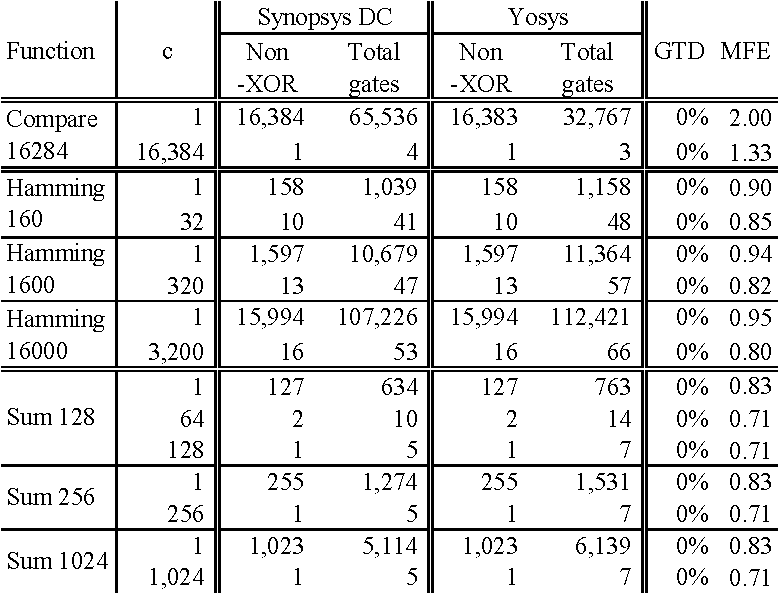
\includegraphics[scale=.9]{abc-crop.pdf}
\end{table}
